% Author: Izaak Neutelings (March 2020)
\documentclass[border=3pt,tikz]{standalone}
\usepackage{amsmath} % for \dfrac
\usepackage{bm} % \bm
\usepackage{physics}
\usepackage{tikz,pgfplots}
\usepackage[outline]{contour} % glow around text
\usetikzlibrary{angles,quotes} % for pic (angle labels)
\usetikzlibrary{calc}
\usetikzlibrary{decorations.markings}
\usetikzlibrary{patterns,snakes}
\tikzset{>=latex} % for LaTeX arrow head
\contourlength{1.6pt}
\usepackage{xcolor}
\colorlet{Bcol}{violet!90}
\colorlet{BFcol}{red!60!black}
\colorlet{Scol}{green!60!black}
\colorlet{veccol}{green!45!black}
\colorlet{Icol}{blue!70!black}
\colorlet{mucol}{red!90!black}
\tikzstyle{BField}=[->,thick,Bcol]
\tikzstyle{current}=[->,Icol] %thick,
\tikzstyle{force}=[->,thick,BFcol]
\tikzstyle{vector}=[->,thick,veccol]
\tikzstyle{mu vector}=[->,thick,mucol]
\tikzstyle{spin}=[->,very thick,Scol]
\tikzstyle{velocity}=[->,very thick,vcol]
\tikzstyle{charge+}=[very thin,draw=black,top color=red!50,bottom color=red!90!black,shading angle=20,circle,inner sep=0.5]
\tikzstyle{charge-}=[very thin,draw=black,top color=blue!50,bottom color=blue!80,shading angle=20,circle,inner sep=0.5]
\tikzstyle{metal}=[top color=black!15,bottom color=black!25,middle color=black!5,shading angle=10]
\tikzset{
  BFieldLine/.style={thick,Bcol,decoration={markings,mark=at position #1 with {\arrow{latex}}},
                                 postaction={decorate}},
  BFieldLine/.default=0.5,
  pics/magnet/.style={ %args={#1}
    code={
      \def\h{0.9}
      \coordinate (-N) at (0,\h);
      \coordinate (-S) at (0,-\h);
      \draw[pic actions,thick,top color=red!60,bottom color=red!90,shading angle=20]
        (-0.8*\h/2,0) rectangle ++(0.8*\h,\h);
      \draw[pic actions,thick,top color=blue!60,bottom color=blue!90,shading angle=20]
        (-0.8*\h/2,0) rectangle ++(0.8*\h,-\h);
      \node[pic actions] at (0, \h/2) {\textbf{N}};
      \node[pic actions] at (0,-\h/2) {\textbf{S}};
  }},
}


\begin{document}


% B FIELD through current loop
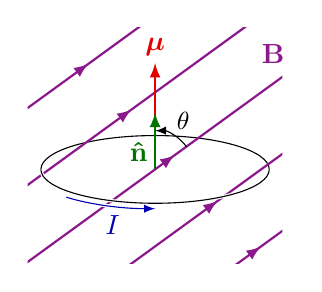
\begin{tikzpicture}
  \def\Rx{1.45}
  \def\Ry{0.43}
  \def\h{0.5}
  \def\H{3}
  \def\L{4}
  \def\NB{5}
  \def\ang{36}
  \coordinate (O) at (0,0);
  \coordinate (N) at (0,0.24*\H);
  \coordinate (M) at (0,0.45*\H);
  \coordinate (B) at (\ang:\H);
  
  % MAGNETIC FIELD
  \draw (-\Rx,0) arc (180:0:{\Rx} and {\Ry});
  \begin{scope}
    \clip ({-0.5*\L*cos(\ang)},-0.4*\H) rectangle ++({\L*cos(\ang)},\H);
    %\foreach \i [evaluate={\y=(\i-0.5)*\H/(\NB-0.5)/2;
    %                       \yl=-\H/2+(\i-0.5)*\H/(\NB-0.5)/2;}] in {1,...,\NB}{
    %  %\draw[BFieldLine,thin] (0,\y)++(\ang-180:0.5*\L) --++ (\ang:\L);
    %  %\draw[BFieldLine,thin] (0,-\y)++(\ang-180:0.5*\L) --++ (\ang:\L);
    %  \draw[BFieldLine,thin] (-\H/2,\y) -- ({-\H/2+(\H/2-\y)*cos(\ang)},\H/2);
    %  \draw[BFieldLine,thin] (-\H/2,-\y) -- ({-\H/2+(\H/2+\y)*cos(\ang)},+\H/2);
    %  \draw[BFieldLine,thin] ({\H/2-(\H/2+\yl)*cos(\ang)},-\H/2) -- (\H/2,\yl);
    %  \draw[BFieldLine,thin] ({\H/2-(\H/2-\yl)*cos(\ang)},-\H/2) -- (\H/2,-\yl);
    %}
    \foreach \i [evaluate={\x=-0.31*\H+(\i-1)*0.62*\H/(\NB-1);
                           \y=-cot(\ang)*\x;
                           \a=0.50+0.017*\i}] in {1,...,\NB}{ %0.58-0.02*(\i-\NB/2-1)^2
      \draw[BFieldLine=\a] (\x,\y)++(\ang-180:\H) --++ (\ang:2*\H);
      %\fill[red] (\x,\y) circle (0.05);
    }
  \end{scope}
  \node[Bcol] at (\H/2,0.49*\H) {$\vb{B}$};
  
  % CIRCUIT
  \draw[white,very thick]
        (-\Rx,0) arc (-180:0:{\Rx} and {\Ry});
  \draw (-\Rx,0) arc (-180:0:{\Rx} and {\Ry});
  %\draw[white,very thick] (0,0) ellipse ({\R} and {0.3*\R});
  %\draw (0,0) ellipse ({\R} and {0.3*\R});
  %\draw (0,0) ellipse ({\R} and {0.3*\R});
  \draw[mu vector] (0,0) -- (M) node[above=-1] {$\vb*{\mu}$};
  \draw[vector] (0,0) -- (N) node[midway,below=4,left=-1] {$\vu{n}$};
  \draw pic[->,"\small$\;\theta$",draw=black,angle radius=14,angle eccentricity=1.4]
    {angle = B--O--N};
  \draw[white,very thick]
    (-150:{1.1*\Rx} and {1.16*\Ry}) arc (-150:-80:{1.1*\Rx} and {1.16*\Ry});
  \draw[current]
    (-135:{1.1*\Rx} and {1.16*\Ry}) arc (-135:-90:{1.1*\Rx} and {1.16*\Ry})
    node[midway,right=2,below] {$I$};
  
\end{tikzpicture}


% MAGNET FIELD through current loop - NS
\def\Rx{0.7}
\def\Ry{1.14}
\def\h{0.5}
\def\H{3}
\def\W{4}
\def\NB{2}
\begin{tikzpicture}
  
  % MAGNETIC
  \draw (0,\Ry) arc (90:270:{\Rx} and {\Ry});
  \foreach \i [evaluate={\y=(0.34*\H)*\i^2/\NB; \in=1*\i^2; \out=180+10*\i^2; \f=0.26+0.10*\i;}] in {1,...,\NB}{
    \draw[BFieldLine=\f] (0.25*\W, \y) to[out= \out,in= \in,looseness=0.8] (-0.95*\H, 0.4*\y/\H);
    \draw[BFieldLine=\f] (0.25*\W,-\y) to[out=-\out,in=-\in,looseness=0.8] (-0.95*\H,-0.4*\y/\H);
  }
  \pic[rotate=90] (M) at (-0.9*\W,0) {magnet};
  \node[Bcol] at (0.26*\W,0.52*\H) {$\vb{B}$};
  
  % CIRCUIT
  \draw[white,very thick]
        (0,\Ry) arc (90:-90:{\Rx} and {\Ry});
  \draw (0,\Ry) arc (90:-90:{\Rx} and {\Ry});
  \draw[mu vector] (0,0) --++ (-0.3*\W,0) node[above left=-3] {\contour{white}{$\vb*{\mu}$}};
  \draw[force] ( 95:{\Rx} and {\Ry}) --++ ( 140:0.7*\Ry) node[left=-1] {\contour{white}{$\vb{F}$}};
  \draw[force] (-95:{\Rx} and {\Ry}) --++ (-140:0.7*\Ry) node[left=-1] {\contour{white}{$\vb{F}$}};
  \draw[current]
    (-70:{1.1*\Rx} and {1.1*\Ry}) arc (-70:-35:{1.1*\Rx} and {1.1*\Ry})
    node[midway,right=2,below] {$I$};
  
\end{tikzpicture}


% MAGNET FIELD through current loop - SN
\begin{tikzpicture}
  
  % MAGNETIC
  \draw (0,\Ry) arc (90:270:{\Rx} and {\Ry});
  \foreach \i [evaluate={\y=(0.34*\H)*\i^2/\NB; \out=1*\i^2; \in=180+10*\i^2; \f=0.80-0.10*\i;}] in {1,...,\NB}{
    \draw[BFieldLine=\f] (-0.95*\H, 0.4*\y/\H) to[out= \out,in= \in,looseness=0.8] (0.25*\W, \y);
    \draw[BFieldLine=\f] (-0.95*\H,-0.4*\y/\H) to[out=-\out,in=-\in,looseness=0.8] (0.25*\W,-\y);
  }
  \pic[rotate=-90] (M) at (-0.9*\W,0) {magnet};
  \node[Bcol] at (0.26*\W,0.52*\H) {$\vb{B}$};
  
  % CIRCUIT
  \draw[force] ( 95:{\Rx} and {\Ry}) --++ (-25:0.8*\Ry) node[right=0] {\contour{white}{$\vb{F}$}};
  \draw[force] (-95:{\Rx} and {\Ry}) --++ ( 25:0.8*\Ry) node[right=1] {\contour{white}{$\vb{F}$}};
  \draw[white,very thick]
        (0,\Ry) arc (90:-90:{\Rx} and {\Ry});
  \draw (0,\Ry) arc (90:-90:{\Rx} and {\Ry});
  \draw[mu vector] (0,0) --++ (-0.3*\W,0) node[above left=-3] {\contour{white}{$\vb*{\mu}$}};
  \draw[current]
    (-14:{1.1*\Rx} and {1.1*\Ry}) arc (-14:14:{1.1*\Rx} and {1.1*\Ry})
    node[midway,right=2] {$I$};
  
\end{tikzpicture}


% SOLENOID
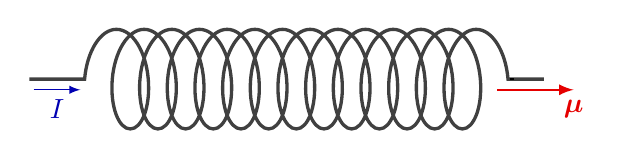
\begin{tikzpicture}[scale=1]
  \def\A{9.0}  % amplitude
  \def\s{10}   % coil segment length
  \def\L{5.4}  % coil length
  \def\a{0.5}  % coil segment aspect
  \def\dy{1.0} % vertical shift
  \def\dx{0.2} % horizontal shift
  \draw[black!75,snake=coil,thick,segment amplitude=2*\A,segment length=\s,segment aspect=\a,very thick]
    (-0.13*\L,0) -- (0,0) -- (\L,0) -- (1.08*\L,0);
  \draw[-,thick]
    (\L,0) -- (1.01*\L,0); % coil extension
  \draw[current] (-0.12*\L,-0.015*\A) --++ (0.11*\L,0) node[midway,below] {$I$};
  \draw[mu vector] (0.97*\L,-0.015*\A) --++ (0.18*\L,0) node[below] {$\vb*{\mu}$};
\end{tikzpicture}


% MAGNETIC MOMENT ATOM
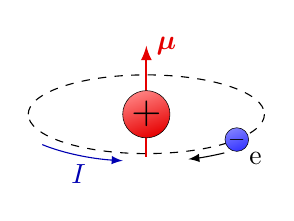
\begin{tikzpicture}
  \def\rn{0.3}
  \def\re{0.15}
  \def\Rx{1.5}
  \def\Ry{0.5}
  %\draw[dashed] (-100:1.5*\rn) -- (80:1.5*\rn);
  \draw[dashed] (-\Rx,0) arc (180:0:{\Rx} and {\Ry});
  \draw[mu vector] (0,-1.8*\rn) -- (0,2.9*\rn) node[right] {$\vb*{\mu}$};
  \draw[charge+] (0,0) circle (\rn) node[scale=1.4] {+};
  \draw[dashed] (\Rx,0) arc (0:-180:{\Rx} and {\Ry});
  \draw[charge-]
    (-40:{\Rx} and {\Ry}) circle (\re) node[scale=0.8] {$-$}
    node[below right=4] {e};
  \draw[->]
    (-55:{1.15*\Rx} and {1.2*\Ry}) arc (-55:-72:{1.15*\Rx} and {1.2*\Ry});
  \draw[current]
    (-140:{1.15*\Rx} and {1.2*\Ry}) arc (-140:-100:{1.15*\Rx} and {1.2*\Ry})
    node[midway,below] {$I$};
\end{tikzpicture}


% MAGNETIC MOMENT ELECTRON
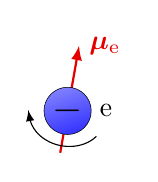
\begin{tikzpicture}
  \def\re{0.3}
  \def\ang{80}
  %\draw[dashed] (\ang-180:2.5*\re) -- (\ang:3.5*\re);
  \draw[mu vector] (\ang-180:1.8*\re) -- (\ang:2.8*\re) node[right] {$\vb*{\mu}_\mathrm{e}$};
  \draw[charge-]
    (0,0) circle (\re) node[scale=1.4] {$-$}
    node[right=10] {e};
  \draw[->,rotate=\ang-90]
    (0,-0.2*\re)++(-30:{1.6*\re} and {1.3*\re}) arc (-30:-165:{1.6*\re} and {1.3*\re})
    --++ (110:0.3*\re);
\end{tikzpicture}


% MAGNETIC MOMENT ELECTRON + SPIN
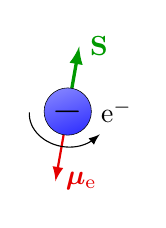
\begin{tikzpicture}
  \def\re{0.3}
  \def\ang{80}
  %\draw[dashed] (\ang-180:2.5*\re) -- (\ang:3.5*\re);
  \draw[mu vector] (0,0) -- (\ang+180:3*\re) node[right] {$\vb*{\mu}_\mathrm{e}$};
  \draw[spin] (0,0) -- (\ang:2.8*\re) node[right] {$\vb{S}$};
  \draw[charge-]
    (0,0) circle (\re) node[scale=1.4] {$-$}
    node[right=10] {$\mathrm{e}^-$};
  \draw[->,rotate=\ang-90]
    (0,-0.2*\re)++(-175:{1.6*\re} and {1.3*\re}) arc (-175:-35:{1.6*\re} and {1.3*\re})
    --++ (50:0.3*\re);
\end{tikzpicture}


% MAGNETIC MOMENT POSITRON + SPIN
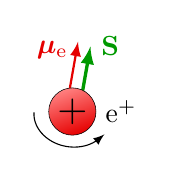
\begin{tikzpicture}
  \def\re{0.3}
  \def\ang{80}
  %\draw[dashed] (\ang-180:2.5*\re) -- (\ang:3.5*\re);
  \draw[mu vector] (-0.28*\re,0) --++ (\ang:3*\re) node[below=3,left=0] {$\vb*{\mu}_\mathrm{e}$};
  \draw[spin] (0.28*\re,0) --++ (\ang:2.8*\re) node[right] {$\vb{S}$};
  \draw[charge+]
    (0,0) circle (\re) node[scale=1.4] {$+$}
    node[right=10] {$\mathrm{e}^+$};
  \draw[->,rotate=\ang-90]
    (0,-0.2*\re)++(-175:{1.6*\re} and {1.3*\re}) arc (-175:-35:{1.6*\re} and {1.3*\re})
    --++ (50:0.3*\re);
\end{tikzpicture}


% MAGNETIC MOMENT FLIP
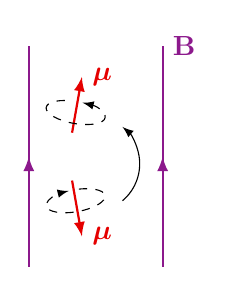
\begin{tikzpicture}
  \def\rm{0.2}
  \def\rx{1.9*\rm}
  \def\ry{0.7*\rm}
  \def\ang{80}
  \def\W{1.7}
  \def\H{2.8}
  \coordinate (T) at (0,0.2*\H);
  \coordinate (B) at (0,-0.2*\H);
  
  % B FIELDS
  \draw[BFieldLine] (-0.35*\W,-\H/2) --++ (0,\H);
  \draw[BFieldLine] ( 0.65*\W,-\H/2) --++ (0,\H) node[right] {$\vb{B}$};
  
  % VECTORS
  \draw[mu vector] (T)++(\ang-180:1.3*\rm) --++ (\ang:3.6*\rm) node[right] {$\vb*{\mu}$}; %_\mathrm{e}
  \draw[mu vector] (B)++(180-\ang:1.3*\rm) --++ (-\ang:3.6*\rm) node[right] {$\vb*{\mu}$};
  \draw[<-,dashed,rotate=\ang-90]
    (T)++(80:{\rx} and {\ry}) arc (80:-260:{\rx} and {\ry});
  \draw[->,dashed,rotate=90-\ang]
    (B)++(80:{\rx} and {\ry}) arc (80:-260:{\rx} and {\ry});
  \draw[->]
    (B)++(0.35*\W,0) arc (-50:50:0.36*\W);
  
\end{tikzpicture}


% LARMOR PRECESSION
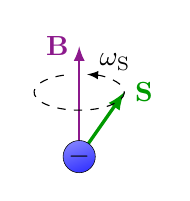
\begin{tikzpicture}
  \def\ang{55}
  \def\S{1.0}
  \def\B{1.4}
  \def\Rx{\S*cos(\ang)}
  \def\Ry{0.4*\Rx}
  \coordinate (O) at (0,0);
  
  \draw[BField] (O) -- (90:\B) node[left] {$\vb{B}$};
  \draw[spin] (O) -- (\ang:\S) node[right] {$\vb{S}$};
  \node[charge-,scale=1] (O) {$-$};
  \draw[->,dashed]
    (0,{\S*sin(\ang)})++(110:{\Rx} and {\Ry}) arc (110:440:{\Rx} and {\Ry})
    node[right=3,above right=-2] {$\omega_\mathrm{S}$};
  
\end{tikzpicture}


\end{document}